\section{Data}
Empirical data for this study was collected from three sources, including two open datasets that are historical records of transactions in the UK\footnote{\textit{HM Land Registry: Price Paid Data}. (2016). [Dataset]. \href{https://www.gov.uk/government/collections/price-paid-data}{https://www.gov.uk/government/collections/price-paid-data}} and Energy Performance Certificates (EPCs) of private domestic dwellings in the UK and Wales\footnote{\textit{Energy Performance of Buildings Data England and Wales}. (n.d.). [Dataset]. Retrieved 16 August 2024, from \href{https://epc.opendatacommunities.org/}{https://epc.opendatacommunities.org/}}; as well as aggregated listing data provided by Zoopla. \footnote{Zoopla Limited, © 2024 2. Zoopla Limited. Economic and Social Research Council. Zoopla Property Data, 2024 [data collection].}
The first two datasets were consolidated and matched by unique property identifiers, called Unique Property Reference Numbers (UPRNs), and two mapping files were downloaded from the University of Glasgow Urban Big Data Centre (UBDC), namely the Price Paid Data to UPRNs \footnote{Urban Big Data Centre (2023). Price paid data to UPRN lookup [Data set]. University of Glasgow. \url{https://doi.org/10.20394/agu7hprj}} and the EPC Individual lodgement identifier (LMK) to UPRNs \footnote{Urban Big Data Centre (2023). Energy Performance Certificate to UPRN lookup [Data set]. University of Glasgow. \url{https://doi.org/10.20394/okfrrz60}}. The linkages above provided an accuracy rate of 96\% \cite{urban_big_data_centre_price_2023}. Outliers occurred where the parent UPRNs (e.g. entire building with a unique address) were not distinct from their child UPRNs (e.g. flats in the building) which resulted in anomalistic amounts of transactions. These occurrences were removed during the data cleaning. The data processing for this study was conducted using RStudio, an integrated development environment (IDE) for R. RStudio was chosen due to its comprehensive suite of tools for data manipulation, statistical analysis, and visualization.

\subsection{Energy Performance Certificates}
\label{EPC_data}
Energy Performance Certificates (EPCs) were introduced in the UK on 1 August, 2007 by the Housing Act 2004 and EPBR 2007. \footnote{The Energy Performance of Buildings (Certificates and Inspections) (England and Wales) Regulations 2007}  Figure \ref{fig:EPC_example} below represents the energy efficiency from a typical certificate processed for this study . 
\begin{figure}[h!]
    \centering
    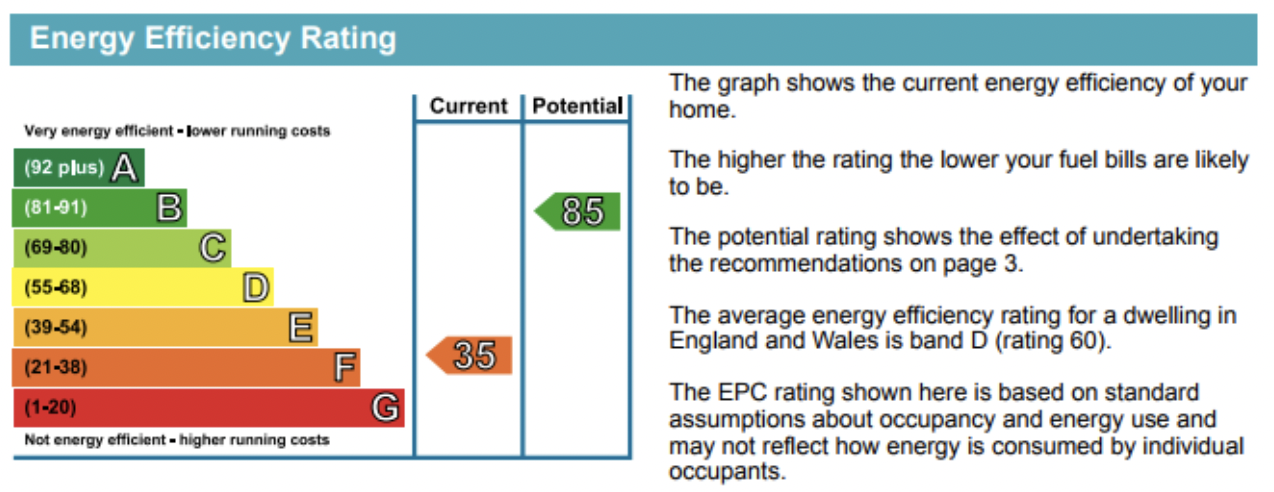
\includegraphics[width=1\linewidth]{src/figures/EPCertificate.png}
    \caption{Typical example of Energy Efficiency Rating reported in an EPC.}
    \label{fig:EPC_example}
\end{figure}
EPCs are determined for a dwelling upon inspection using the Standard Assessment Procedure (SAP). The SAP and RdSAP (Reduced SAP) methodologies are developed by an external organization - the Building Research Establishment (BRE) - and have been criticised for estimating the cost-efficiency - rather than energetic performance - of buildings \cite{kelly_building_2012}. Since SAP ratings mostly take into account energy appliances and house geometry (as estimators of energy use) \cite{department_for_communities_and_local_government_guide_2017, bre_group_standard_nodate} they can overlook the 'fabric' energy efficiency \cite{bolton_energy_2024} \footnote{refers to passive characteristics of buildings which affect energy efficiency, such as insulation} of buildings and may hence not act as the most efficient predictors of carbon emissions \cite{stone_key_2014}. Studies comparing smart meters and domestic EPC energy use ratings have also shown discrepancies in estimations, specially significant over-predictions of energy use in lower rated dwellings due to assumptions on building characteristics and occupancy in the SAP modelling \cite{few_over-prediction_2023}. Other findings suggest this 'measurement error' results in less-accurate estimations in Bands C and lower due to the increase variance in repeated measurements \cite{crawley_quantifying_2019}. Energy-poor properties tend to be the most significantly impacted by the lack of consistency and accuracy of EPC ratings. To avoid these errors, some studies restricted their sample to Bands D and above \cite{ghosh_homebuyers_2024} when attempting to estimate consumer's willingness to pay for energy efficiency. However, this study aims to explore the inequalities and aggregate impacts of improving the housing sector to their maximum potential energy efficiency, which inevitably will affect the lower-rated dwellings. Additionally, when estimating the green premium (see \ref{Sec:green_premium} ) of green-labelled dwellings, it has been shown that government endorsement, simplicity, and financial incentives are key factors determining the trust in certificates rather than the accuracy of the latter \cite{banerjee_eco-labeling_2003, mutter_increasing_2012, martiskainen_role_2019}. Therefore, while there are shortcomings to the SAP methodology, its wide application serves a consistent and standardized index of energy use, sufficient for the purpose of investigating market responses to consumer awareness and policy-incentives. \\


The energy efficiency ratings of 15 million dwellings were extracted from Energy Performance Certificates (EPC) available on the Energy Performance of Buildings Register ('the register' ). Since 2008, all properties listed for sell, rent, or newly constructed must undergo an inspection \cite{department_for_communities_and_local_government_guide_2017}. A certified assessor assigns an energy efficiency ratings from the Standard Assessment Procedure (SAP) in newly built homes and Reduced SAP (RdSAP) in retrofitted homes \cite{department_for_energy_security_and_net_zero_and_department_for_business_energy__industrial_strategy_standard_2013, department_for_energy_security_and_net_zero_and_department_for_business_energy__industrial_strategy_standard_2023}. SAP energy ratings are determined from an estimated ratio of energy consumption and production for each property and provide an energy cost factor on a scale of 1 to 100 (or above 100 if a site generates more energy than it needs) \cite{bre_group_standard_nodate, bolton_energy_2024}. The given numerical scores can be converted to ABCDG bands of energy efficiency - from least efficient and high running costs (1-20 : G) to most energy efficient and low running costs (92+ : A). EPCs provide additional information on the insulation and efficiency of all elements of the property, heating methods, estimated energy needs/costs, and carbon emissions, as well as more detailed information about the properties (such as property size, building age and other property characteristics). After selecting for the observations that could improve their EPC and cleaning the dataset, $15,602,800$ dwellings were kept and analysed as they were able to reach the minimum EPC rating standards imposed by the PRS.

\begin{figure}[h!]
    \centering
    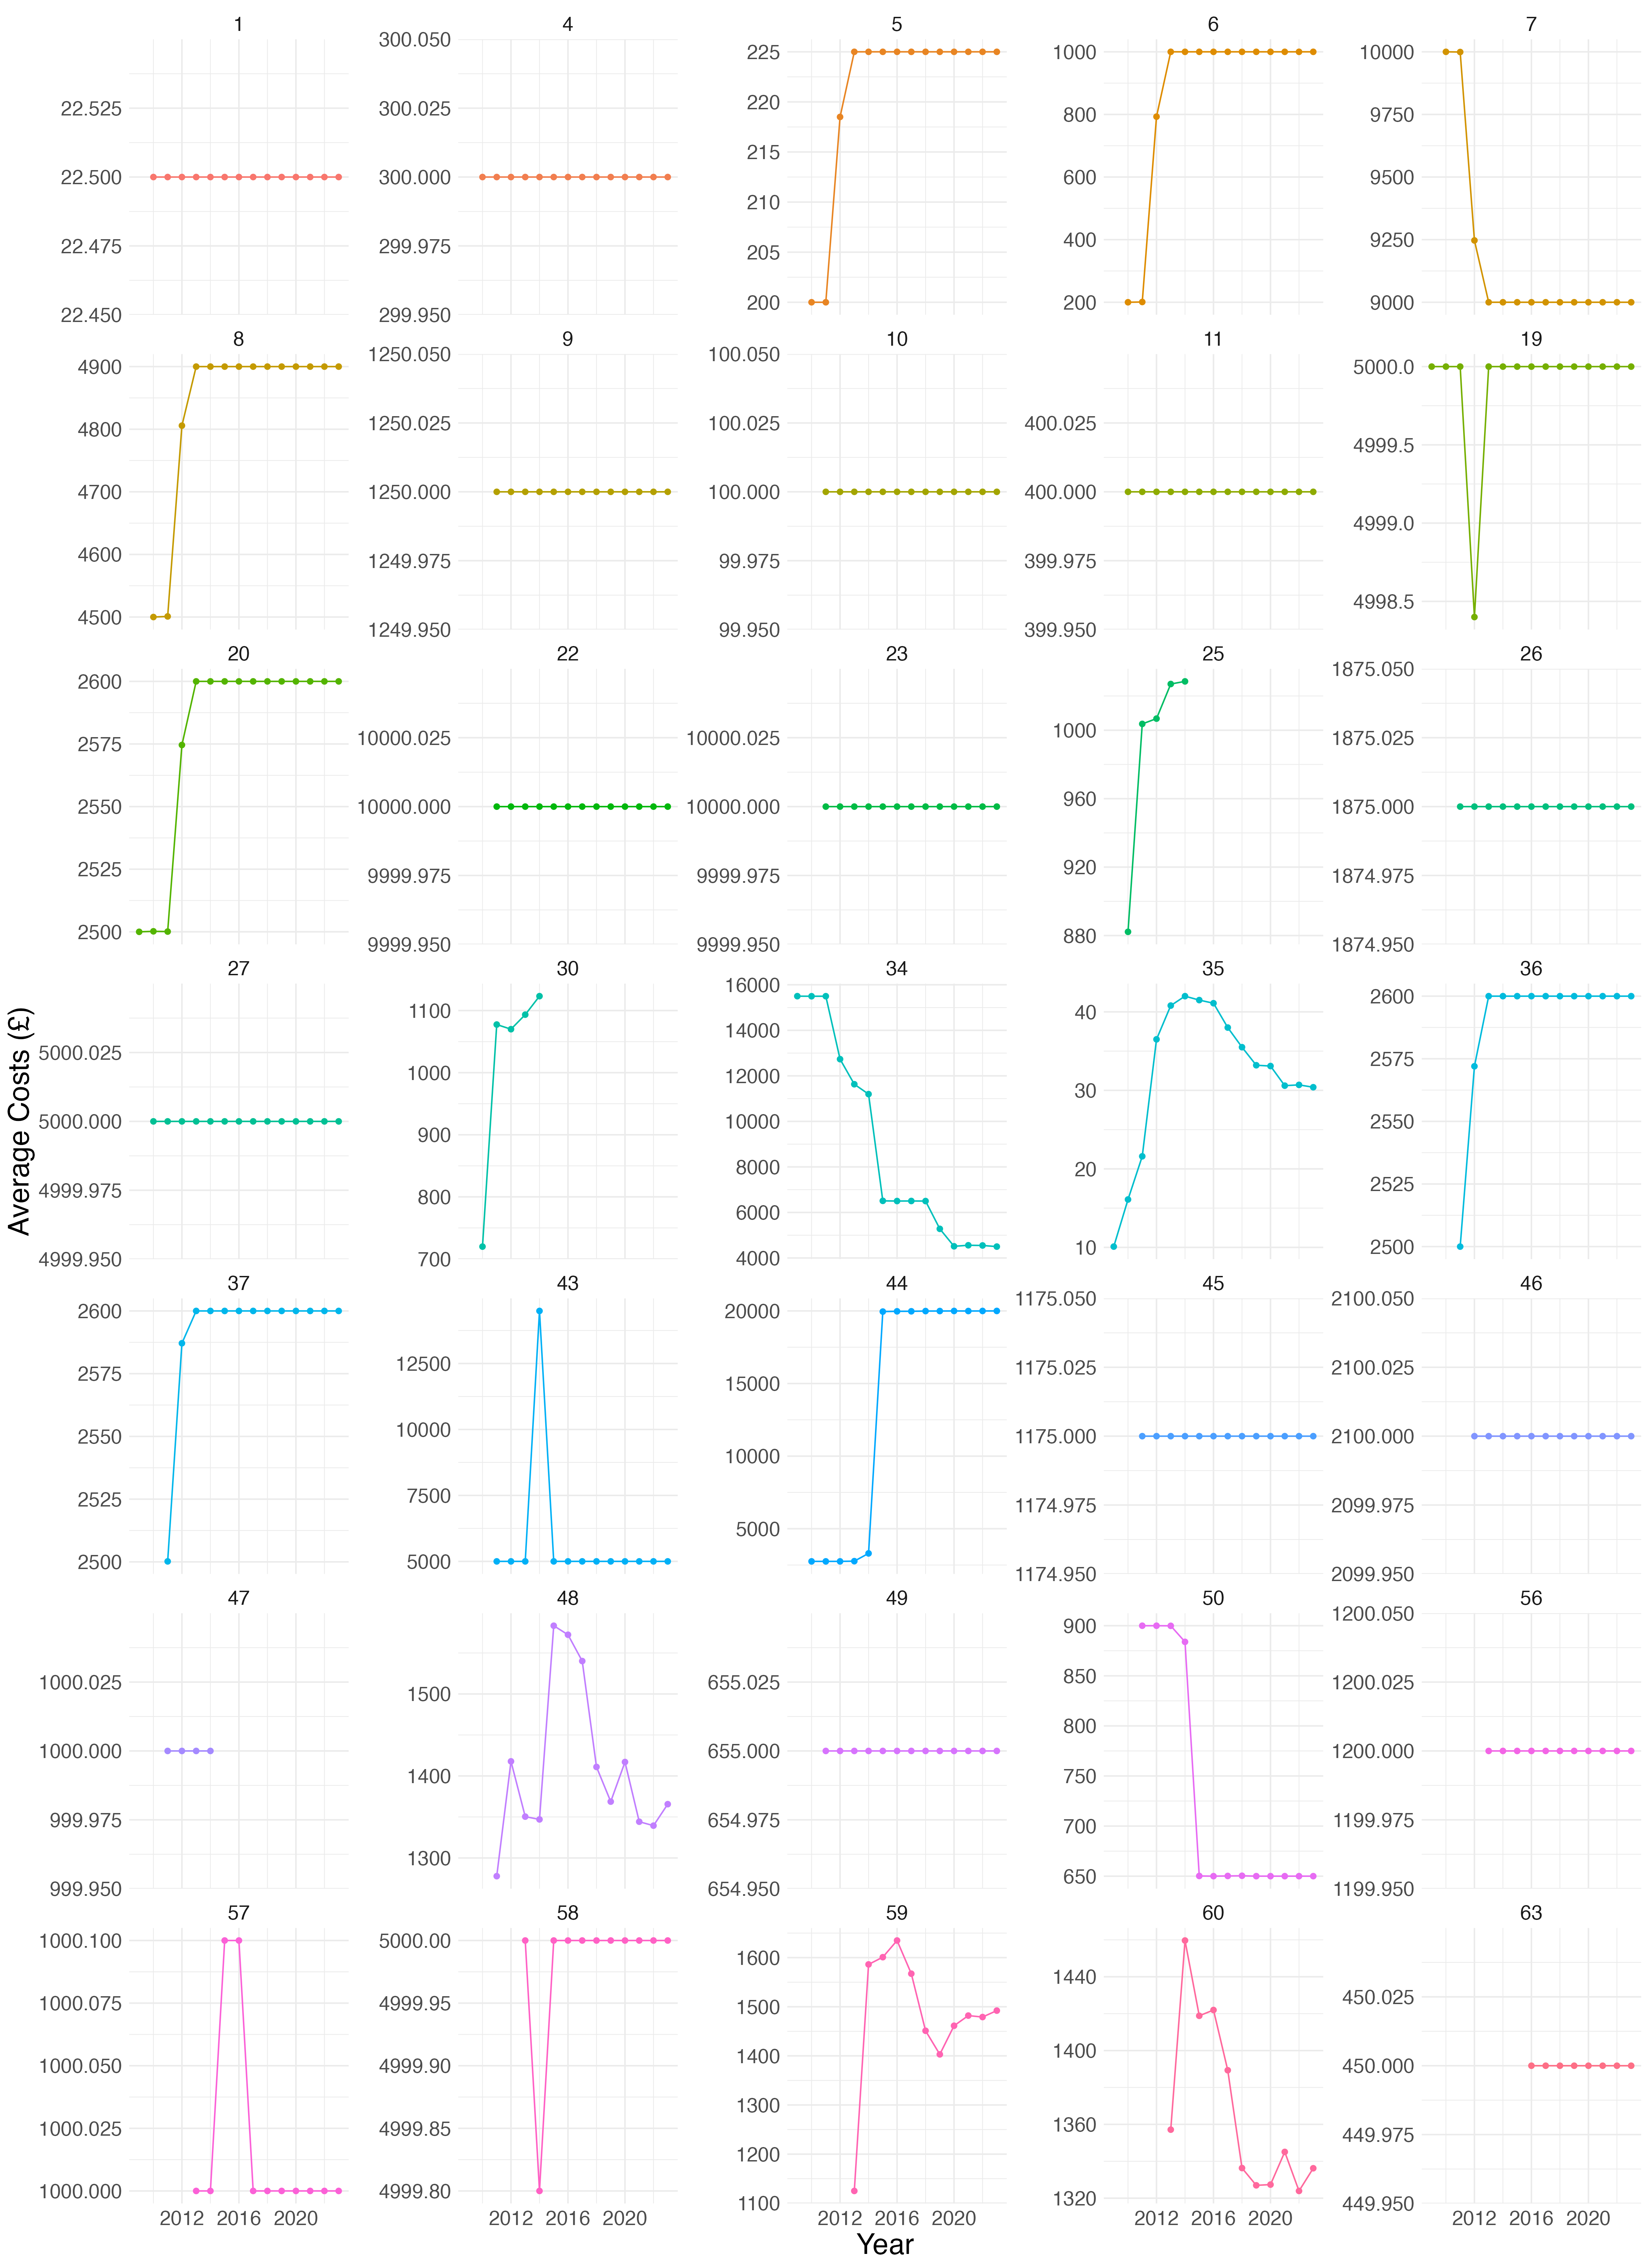
\includegraphics[width=1\textwidth]{src/figures/Facet_costs.png} % Adjust width as needed
    \caption{Average Yearly Costs by Improvement ID, extracted from EPC recommendations for all dwellings let, sold or retrofitted between 2008 - 2023}
    \label{fig:facet_price}
\end{figure}

\subsection{Price Paid Data and Listing Dataset} 
The HM Land Registry's Price Paid data provides nearly a full record of all residential property sales in England and Wales since 1995.\footnote{\textit{HM Land Registry: Price Paid Data}. (2016). [Dataset]. \href{https://www.gov.uk/government/collections/price-paid-data}{https://www.gov.uk/government/collections/price-paid-data}} Transactions excluded from the Price Paid Data are homes not registered with the HM Land Registry and all unorthodox transfer of property rights (i.e., Deeds, 'Right to Buy' discounted properties, etc.). While previously only commercially available, the UK Land Registry data became accessible to the public as of 2013, making historical records of cash and mortgage transactions open data. For the purpose for this study, variables included the transaction prices, date, location (by postcode), property type, and UPRNs. In total 14.5 million transactions were extracted from the Price Paid data between 2007-23, of which 9.6 million consisted of unique addresses (or UPRNs). \\

\begin{table}[!h]
\centering
\caption{Summary Statistics of average transaction price by property type and EPC rating as defined by RdSAP.}
\begin{tabular}{lrrrrr}
\toprule
EPC Rating & Bungalow & Flat & House & Maisonette & Park home\\
\midrule
\cellcolor{gray!10}{A} & \cellcolor{gray!10}{297144.7} & \cellcolor{gray!10}{328078.0} & \cellcolor{gray!10}{366825.9} & \cellcolor{gray!10}{384231.6} & \cellcolor{gray!10}{-}\\
B & 298159.8 & 297840.0 & 304817.2 & 342341.8 & -\\
\cellcolor{gray!10}{C} & \cellcolor{gray!10}{279565.3} & \cellcolor{gray!10}{228881.0} & \cellcolor{gray!10}{264755.1} & \cellcolor{gray!10}{254608.2} & \cellcolor{gray!10}{278219.6}\\
D & 264678.9 & 243516.0 & 264634.6 & 273549.8 & 184001.2\\
\cellcolor{gray!10}{E} & \cellcolor{gray!10}{274003.5} & \cellcolor{gray!10}{238571.2} & \cellcolor{gray!10}{283038.0} & \cellcolor{gray!10}{269317.8} & \cellcolor{gray!10}{246575.5}\\
\addlinespace
F & 277801.3 & 211757.1 & 299006.1 & 235927.6 & 226707.8\\
\cellcolor{gray!10}{G} & \cellcolor{gray!10}{256178.3} & \cellcolor{gray!10}{206546.6} & \cellcolor{gray!10}{240768.1} & \cellcolor{gray!10}{218924.4} & \cellcolor{gray!10}{291646.8}\\
\bottomrule
\label{Descriptive_Price}
\end{tabular}
\end{table}


Transaction prices were adjusted for inflation using the Retail Price Index (RPI) for the sample period which was sourced from the Office of National Statistics (ONS) \footnote{https://www.ons.gov.uk/economy/inflationandpriceindices}. While the Consumer Price Index (CPI) has been the prevailing inflation index in the UK since 2003, after its inception in 1996 \cite{office_for_national_statistics_ons_consumer_2023},  both indicators rely on the overall change in price paid by households for the goods and services they consume \cite{jonhson_uk_2015}. However, they differ in the 'basket of goods (data) and formula used \cite{levell_comparing_2012}. As seen in Figure~\ref{fig:RPIvCPI} in Appendix, the RPI relies more heavily on housing expenditures (e.g., housing purchase costs, mortgage interest payments, building insurance, etc.) making it more sensitive to housing market conditions \cite{levell_comparing_2012}. This is especially relevant during the subprime mortgage crisis, as the RPI provided a significantly better representation of the turbulent housing prices therefore, the "real" transaction prices were adjusted from the RPI as of January 2019. Properties in the top 1\% of transaction prices were considered luxury goods and hence removed from the panel of observations since they are subject to distinct consumer behaviours \cite{allsopp_additional_2005} which may directly affect the willingness to pay for certain characteristics and services such as green labels \cite{fuerst_green_2016, hui_housing_2021, fuerst_energy_2016} hence affecting the underlying trends investigated here.  \\



Finally, access to rental and sales Zoopla property data from 2016-22 were granted by Zoopla Limited\footnote{Zoopla Limited, © 2024 2. Zoopla Limited. Economic and Social Research Council. Zoopla Property Data, 2024} under licensed agreement and aggregated at postcode level each property in order to control for variations in supply in the housing market across the UK and Wales. For each property, the time period listed on the market until sold or rented was provided enabling the computation of the active listings in an area surrounding a point of transaction. For each listing period, the number of listings was therefore computing across district areas and added as controls for supply. Figure \ref{fig:active_listings} provides an overview of the supply of private homes for rent and sale as aggregated therein, as measured in the number of active listings in a given area and month, showing clear evidence of seasonal trends.

\begin{figure}[h]
    \centering
    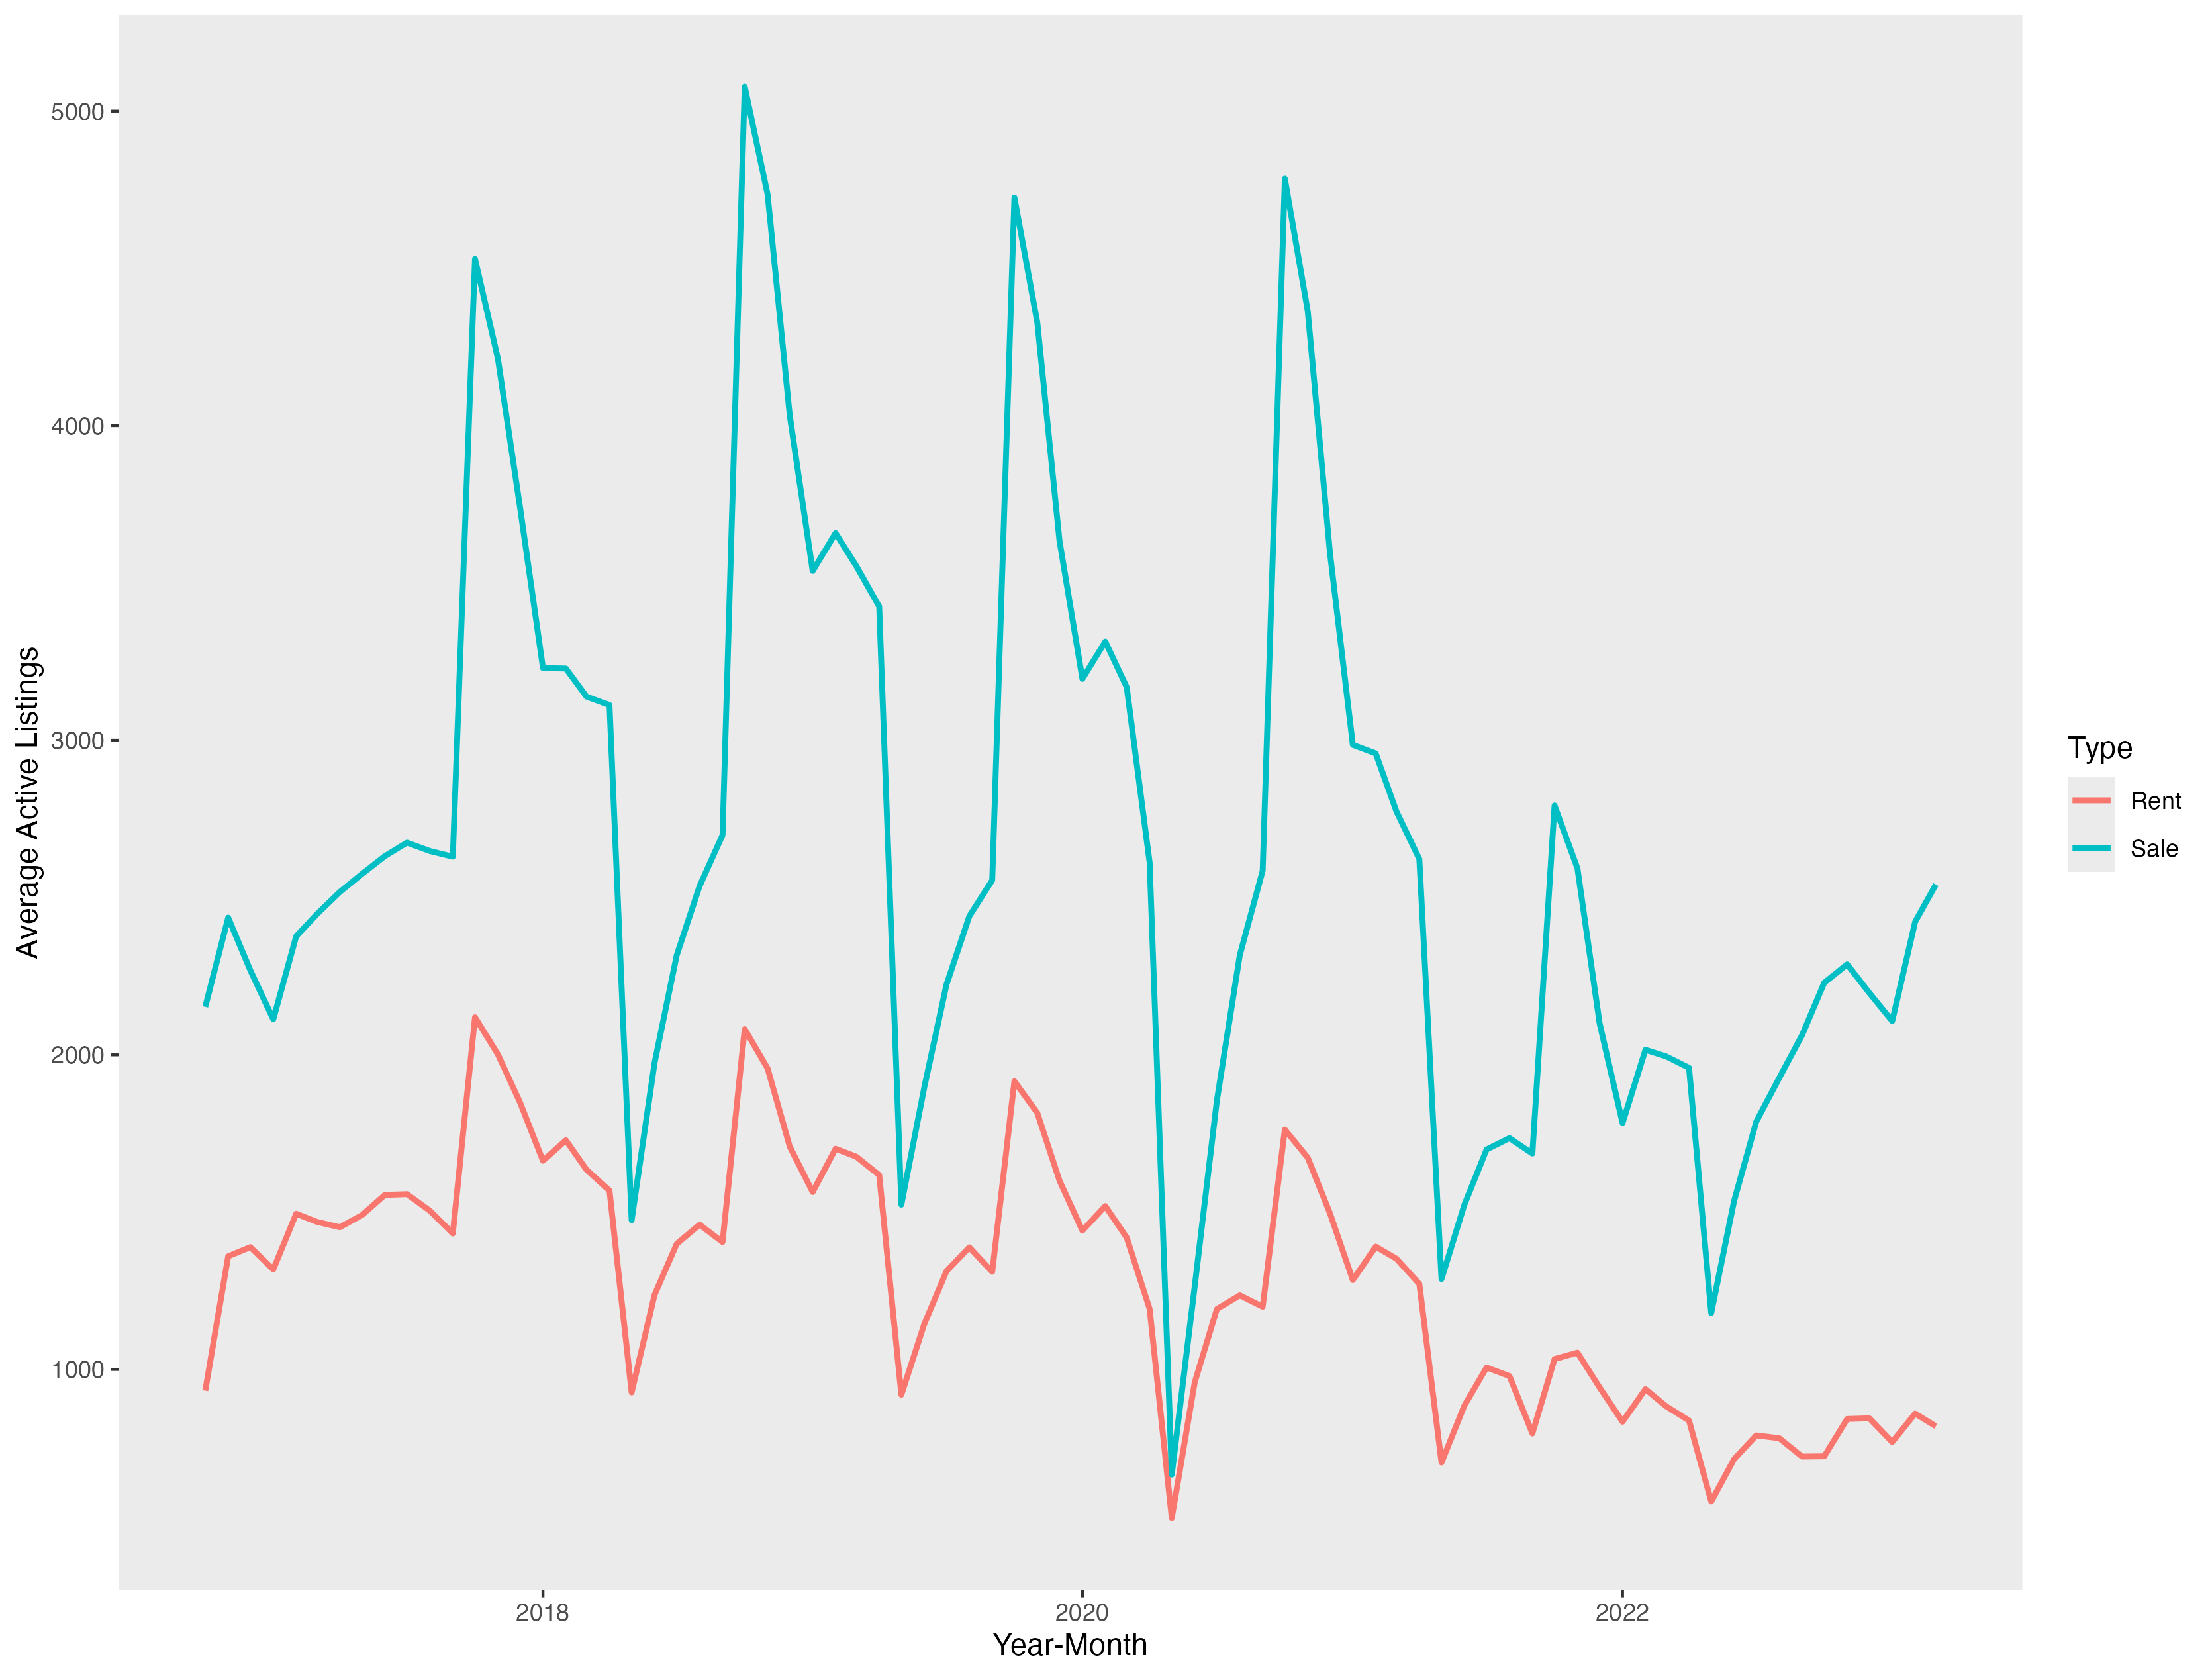
\includegraphics[width=0.75\linewidth]{src/figures/active_listings.png}
    \caption{Average monthly rental and sale active listings in UK and Wales.}
    \label{fig:active_listings}
\end{figure}

